\documentclass[a4paper,11pt,twocolumn]{article}
\usepackage{graphicx,epsfig}
\usepackage{natbib}
\usepackage{hyperref} 
\usepackage{times}
\usepackage[leftcaption]{sidecap}
\usepackage{fancyhdr}
\usepackage{subfigure}      % figures can have sub chunks
\usepackage{geometry}       % this maxes page usage, making the below unnecessary
\usepackage[cc]{titlepic}   % allows a pic to be included in the title page
\usepackage[toc,page]{appendix} % allows for an appendix section
\usepackage[normalem]{ulem} % for table
\useunder{\uline}{\ul}{}    % for table

\textwidth = 6.75in
\oddsidemargin = -0.25in
\textheight = 10in
\topmargin = -0.5in

% definitions for fancyhdr package
\pagestyle{fancy}
\lhead{{\it A. Jaamour, A. Lissak}}
\chead{Computer Vision}
\rhead{CM30080 Coursework}
\lfoot{}
\cfoot{\thepage}
\rfoot{}

\newcommand{\goodgap}{
 \hspace{\subfigtopskip}
 \hspace{\subfigbottomskip}
}

\title{Filtering, Object Recognition and Features}
\author{Adam Jaamour, Andrea Lissak}

\renewcommand{\familydefault}{lmss}
%beautiful table
\usepackage[table]{xcolor}
\usepackage{longtable}
\usepackage{tabularx}
%\setlist{nolistsep}
\definecolor{orange}{HTML}{cd8641}
\definecolor{yellow}{HTML}{f0f4b2}
\definecolor{bordeaux}{HTML}{641113}

%%%%%%%%%%%%%%%%%%%%%%%%%%%%%%%%%%%%%%%%%%%%%%%%%%%%%%%%%%%%%%%%%%%%%%%%
%%%%%%%%%%%%%%%%%%%%%%%%%%%%%%%%%%%%%%%%%%%%%%%%%%%%%%%%%%%%%%%%%%%%%%%%
%%%%%%%%%%%%%%%%%%%%%%%%%%%%%%%%%%%%%%%%%%%%%%%%%%%%%%%%%%%%%%%%%%%%%%%%

\begin{document}
\maketitle
\clearpage

\section{Introduction}

For this project, the programming language of choice was Python. It was chosen over MATLAB due to the availability of functions similar to MATLAB's functions through libraries, and due to the syntax and flexibility of the language. With libraries such as OpenCV for image manipulations \citep{opencv}, Numpy \citep{numpy} and SciPy for more advanced mathematical functions including array manipulations, and MatPlotLib for plotting data \citet{matplotlib}, Python has all the tools for the task at hand.

%%%%%%%%%%%%%%%%%%%%%%%%%%%%%%%%%%%%%%%%%%%%%%%%%%%%%%%%%%%%%%%%%%%%%%%%
%%%%%%%%%%%%%%%%%%%%%%%%%%%%%%%%%%%%%%%%%%%%%%%%%%%%%%%%%%%%%%%%%%%%%%%%
%%%%%%%%%%%%%%%%%%%%%%%%%%%%%%%%%%%%%%%%%%%%%%%%%%%%%%%%%%%%%%%%%%%%%%%%

\section{Convolution Filtering}

A function to perform convolution on an image was written, which adds padding to the edges of the original image in order to preserve image size.

Multiple filters are used to test the convolution function, including:
\begin{enumerate}
    \item Gaussian kernel,
    \item Sharpen kernel,
    \item Horizontal Edge detector (Sober filter),
    \item Identity matrix.
\end{enumerate}

To confirm that the results are correct, the resulting filtered image compared to a library function. SciPy's ``\textit{convolve}'' function was used to carry out this task \citep{scipy-convolve} as it is the equivalent of MATLAB's ``\textit{conv2}'' function. The comparison is done by subtracting  the function's result from the library's result and checking that all the values are equal to 0.

%%%%%%%%%%%%%%%%%%%%%%%%%%%%%%%%%%%%%%%%%%%%%%%%%%%%%%%%%%%%%%%%%%%%%%%%
%%%%%%%%%%%%%%%%%%%%%%%%%%%%%%%%%%%%%%%%%%%%%%%%%%%%%%%%%%%%%%%%%%%%%%%%
%%%%%%%%%%%%%%%%%%%%%%%%%%%%%%%%%%%%%%%%%%%%%%%%%%%%%%%%%%%%%%%%%%%%%%%%

\section{Intensity-Based Template Matching}

\subsection{Pre-Processing}

\begin{enumerate}
    \item setting the image background to 0
    \item normalising each training image
    \item using RGB channels for the image rather than converting to grey scale to avoid losing accuracy
\end{enumerate}

\subsection{Gaussian Pyramids}

\begin{enumerate}
    \item Choice of scale and rotations
    \item A subsampling function was written to recursively scale the image down by half. The Gaussian blur used has a size of 5x5 and a standard deviation of 15. 
    \item templates saved in binary ``\textit{.dat}'' files for quicker I/O operations.
\end{enumerate}

\section{Output: Result Evaluation}

\subsection{Testing and Box Drawing}

Each template for a single class is sled over a an image from the test dataset. Once the similarity score is calculated for each template using Equation \ref{eq:corr}, the template with the highest score for a class is kept if it is higher or equal to a threshold that is set empirically (set at 0.5). This step was repeated for each class.\\

\begin{equation}
\label{eq:corr}
    cor(x,y) = \sum_{i,j} T(i,j) I(i+x, j+y)
\end{equation}

Next, a box along with the class name (rather than class number for clarity) is drawn at the location where the template with the highest score was previously calculated, using the scaling and the rotation of the selected template to draw the rectangle at the correct scale and at the correct rotation. An example can be seen in Figure \ref{fig:template-matching-output-example}.\\

\begin{figure}[!htbp]
\centering
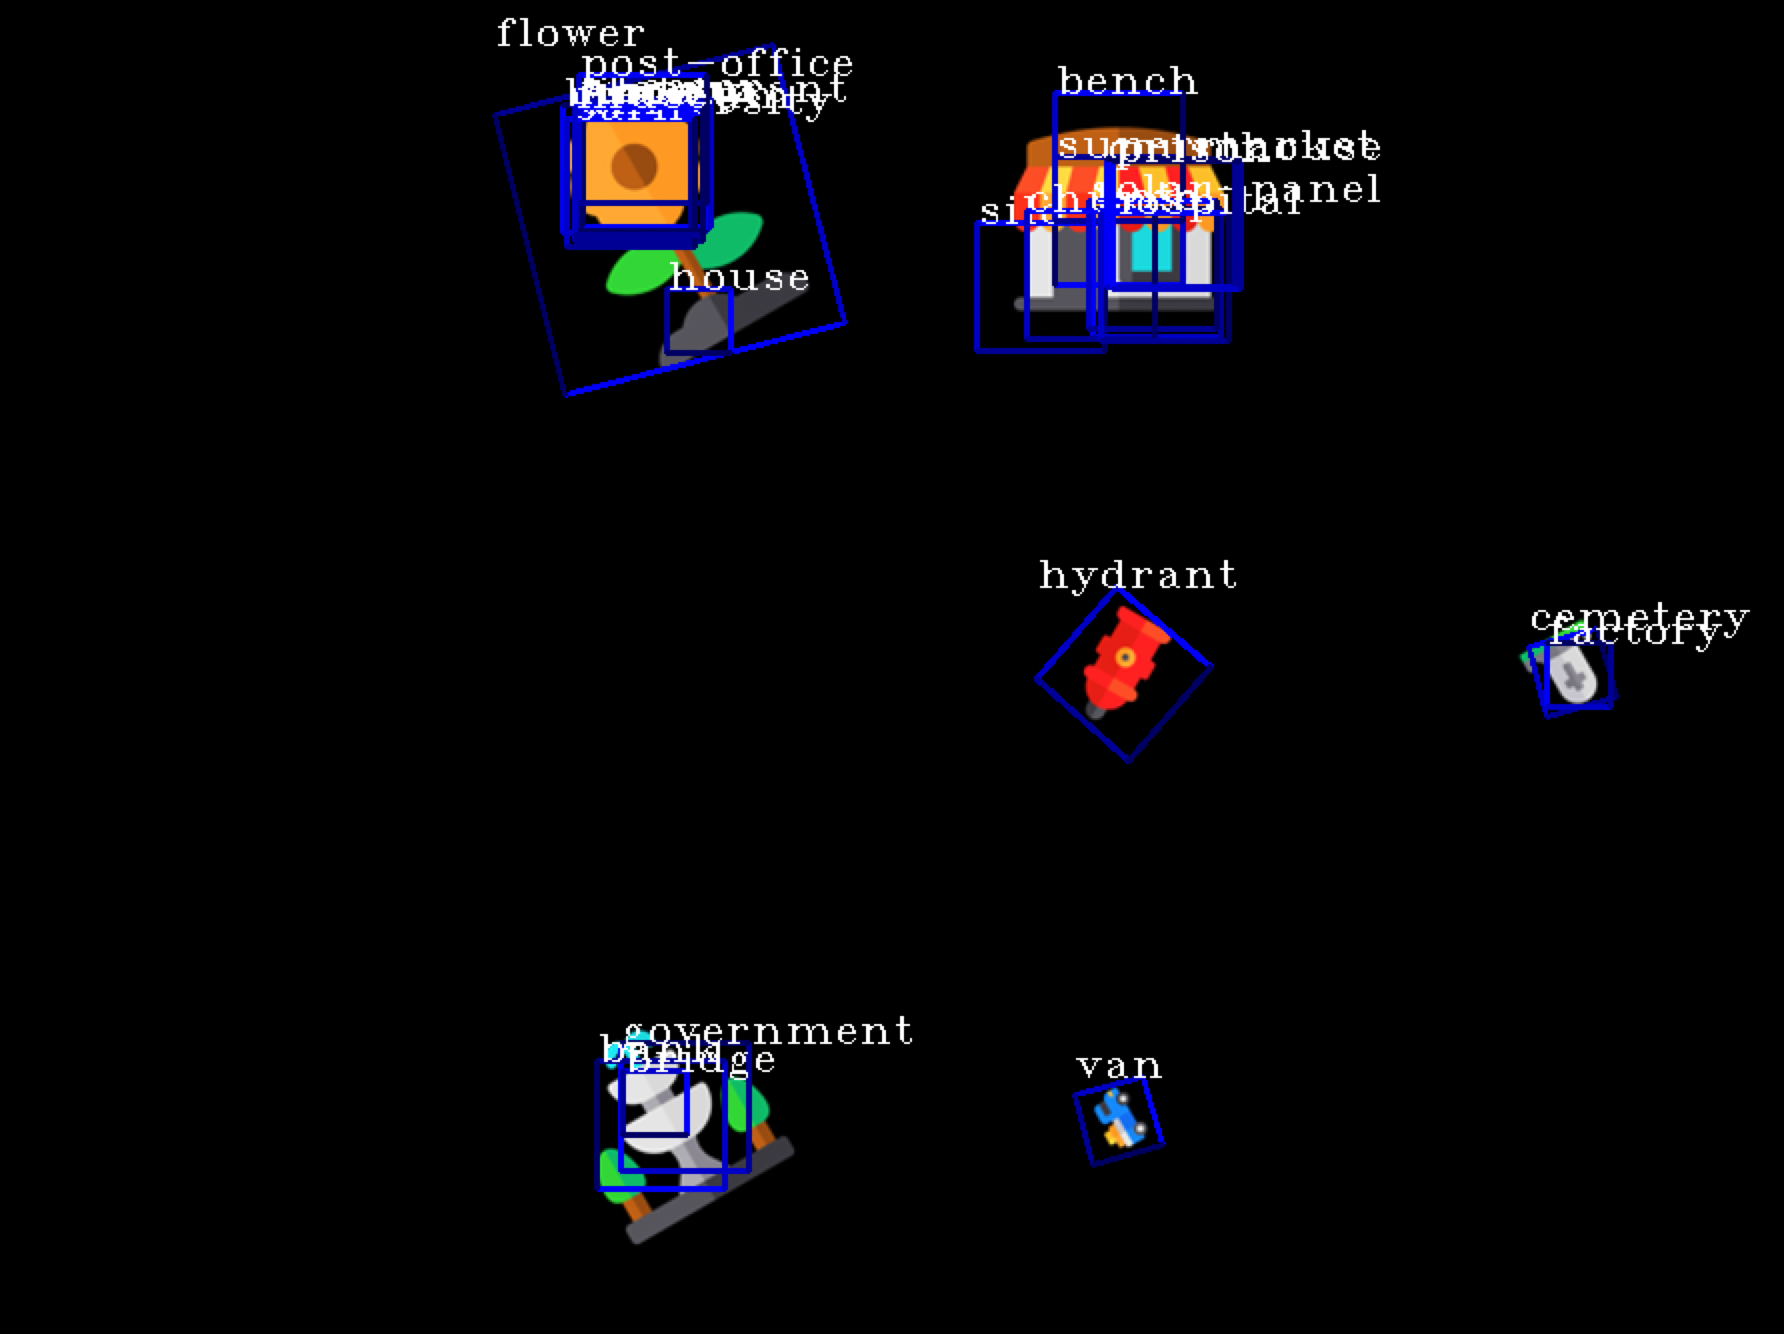
\includegraphics[scale=0.25]{figures/template-matching-output-example.png}
\caption{Example output of Task 2.}
\label{fig:template-matching-output-example} 
\end{figure}

\subsection{Evaluation}

\begin{enumerate}
    \item count the number of false positives and false negatives on all test images (put data in a table or graph). Describe how the choice of the parameters mentioned in the previous sections were to minimise these false positives and false negatives.
    \item calculate average run time for each test and report too.
    \item insights about complexity (memory and runtime) in terms of problem size (3 times more work due to using RGB channel instead of grey scale)
    \item mention scalability
\end{enumerate}

%%%%%%%%%%%%%%%%%%%%%%%%%%%%%%%%%%%%%%%%%%%%%%%%%%%%%%%%%%%%%%%%%%%%%%%%
%%%%%%%%%%%%%%%%%%%%%%%%%%%%%%%%%%%%%%%%%%%%%%%%%%%%%%%%%%%%%%%%%%%%%%%%
%%%%%%%%%%%%%%%%%%%%%%%%%%%%%%%%%%%%%%%%%%%%%%%%%%%%%%%%%%%%%%%%%%%%%%%%

\section{SIFT Features}

\subsection{Pre-processing}

\begin{enumerate}
    \item Describe how the SIFT descriptors were created.
    \item quote Lowe.
\end{enumerate}

\subsection{Output and Result Evaluation}

todo

%%%%%%%%%%%%%%%%%%%%%%%%%%%%%%%%%%%%%%%%%%%%%%%%%%%%%%%%%%%%%%%%%%%%%%%%
%%%%%%%%%%%%%%%%%%%%%%%%%%%%%%%%%%%%%%%%%%%%%%%%%%%%%%%%%%%%%%%%%%%%%%%%
%%%%%%%%%%%%%%%%%%%%%%%%%%%%%%%%%%%%%%%%%%%%%%%%%%%%%%%%%%%%%%%%%%%%%%%%

\section{Discussion \& Conclusion}

Describe how it could have been improved:
\begin{enumerate}
    \item for intensity-based template matching, a box should be drawn for only the best matching template around a location with an object.
\end{enumerate}

%%%%%%%%%%%%%%%%%%%%%%%%%%%%%%%%%%%%%%%%%%%%%%%%%%%%%%%%%%%%%%%%%%%%%%%%
%%%%%%%%%%%%%%%%%%%%%%%%%%%%%%%%%%%%%%%%%%%%%%%%%%%%%%%%%%%%%%%%%%%%%%%%
%%%%%%%%%%%%%%%%%%%%%%%%%%%%%%%%%%%%%%%%%%%%%%%%%%%%%%%%%%%%%%%%%%%%%%%%

\raggedright
\bibliographystyle{apalike}
\bibliography{bibliography}

\onecolumn
\clearpage
\begin{appendices}

% table of contributions
\chapter{Table of Contributions}
\begin{table}[h]
\resizebox{\textwidth}{!}{%
\begin{tabular}{|r|c|c|}
\hline
\textbf{Student Name}            & {\ul Adam Jaamour}                                                                                                                      & {\ul Andrea Lissak}                                                                                                             \\ \hline
\textbf{Student Username}        & \textit{aj645}                                                                                                                          & \textit{al746}                                                                                                                  \\ \hline
\textbf{Student ID}              & \textit{159327001}                                                                                                                      & \textit{159044728}                                                                                                              \\ \hline
\textbf{Contributions}           & \multicolumn{1}{l|}{\textit{\begin{tabular}[c]{@{}l@{}}- Convolution\\ - intensity-based template \\   matching training\end{tabular}}} & \multicolumn{1}{l|}{\textit{\begin{tabular}[c]{@{}l@{}}- SIFT\\ - intensity-based template \\   matching testing\end{tabular}}} \\ \hline
\textbf{Contribution Percentage} & \textit{50\%}                                                                                                                           & \textit{50\%}                                                                                                                   \\ \hline
\end{tabular}%
}
\end{table}

% code snippets

\end{appendices}
\end{document}